\documentclass[11pt,a4paper]{article}

% ---------------------------------------------------------------------------
% PACKAGES
% ---------------------------------------------------------------------------
\usepackage[utf8]{inputenc}
\usepackage[T1]{fontenc}
\usepackage{lmodern}
\usepackage{microtype}
\usepackage[margin=2.54cm]{geometry}
\usepackage{setspace}
\usepackage{titlesec}
\usepackage{abstract}
\usepackage{booktabs}
\usepackage{tabularx}
\usepackage{multirow}
\usepackage{graphicx}
\usepackage{xcolor}
\usepackage{amsmath}
\usepackage{amssymb}
\usepackage{hyperref}
\usepackage{url}
\usepackage{natbib}
\usepackage{pgfplots}
\usepackage{pgfplotstable}
\usepackage{tikz}
\usepackage{caption}
\usepackage{subcaption}
\usepackage{float}
\usepackage{enumitem}
\usepackage{fancyhdr}
\usepackage{lastpage}
\usepackage{datetime}

\pgfplotsset{compat=1.18}

% ---------------------------------------------------------------------------
% COLOURS
% ---------------------------------------------------------------------------
\definecolor{tfidfblue}{RGB}{31, 119, 180}
\definecolor{embedorange}{RGB}{255, 127, 14}
\definecolor{hybridgreen}{RGB}{44, 160, 44}
\definecolor{rwred}{RGB}{214, 39, 40}
\definecolor{enpurple}{RGB}{148, 103, 189}
\definecolor{mixedbrown}{RGB}{140, 86, 75}
\definecolor{accentgray}{RGB}{90, 90, 90}

% ---------------------------------------------------------------------------
% HYPERREF SETUP
% ---------------------------------------------------------------------------
\hypersetup{
  colorlinks = true,
  linkcolor  = tfidfblue,
  citecolor  = tfidfblue,
  urlcolor   = tfidfblue,
  pdftitle   = {KinyaSearch},
  pdfauthor  = {NIYIBIZI Prince},
}

% ---------------------------------------------------------------------------
% HEADER / FOOTER
% ---------------------------------------------------------------------------
\pagestyle{fancy}
\fancyhf{}
\renewcommand{\headrulewidth}{0.4pt}
\fancyhead[L]{\small\textit{KinyaSearch: Kinyarwanda-English Code-Switched Product Search}}
\fancyhead[R]{\small NIYIBIZI Prince}
\fancyfoot[C]{\small\thepage}

% ---------------------------------------------------------------------------
% SECTION TITLE FORMATTING
% ---------------------------------------------------------------------------
\titleformat{\section}{\large\bfseries}{\thesection.}{0.5em}{}
\titleformat{\subsection}{\normalsize\bfseries}{\thesubsection}{0.5em}{}
\titlespacing{\section}{0pt}{14pt}{6pt}
\titlespacing{\subsection}{0pt}{10pt}{4pt}

% ---------------------------------------------------------------------------
% CAPTION STYLE
% ---------------------------------------------------------------------------
\captionsetup{
  font       = small,
  labelfont  = bf,
  labelsep   = period,
  justification = raggedright,
  singlelinecheck = false,
}

% ---------------------------------------------------------------------------
% DOCUMENT
% ---------------------------------------------------------------------------
\begin{document}

% ============================================================
% TITLE BLOCK
% ============================================================
\begin{center}

{\LARGE\bfseries KinyaSearch: The First Benchmark Dataset and\\[4pt]
Retrieval System for Kinyarwanda-English\\[4pt]
Code-Switched Product Search}

\vspace{18pt}

{\large NIYIBIZI Prince}\\[4pt]
{\normalsize Taizhou University}\\[2pt]
{\normalsize \href{mailto:princeniyibizi4@gmail.com}{princeniyibizi4@gmail.com}}

\vspace{10pt}
{\normalsize May 2026}

\end{center}

\vspace{12pt}
\hrule
\vspace{12pt}

% ============================================================
% ABSTRACT
% ============================================================
\begin{abstract}
\noindent
We present KinyaSearch — a hybrid information retrieval system built for
Kinyarwanda-English code-switched e-commerce queries, a problem that
existing multilingual search infrastructure handles poorly or not at all.
The system combines a bilingual TF-IDF index with multilingual sentence
embeddings from \texttt{paraphrase-multilingual-MiniLM-L12-v2}, fusing
both signals through a weighted linear scoring function. Alongside the
system, we release the first publicly available Kinyarwanda e-commerce
benchmark: a 60-product bilingual catalog, a 90-query evaluation set
spanning pure Kinyarwanda, pure English, and code-switched queries, and
a 68-term Kinyarwanda commerce vocabulary lexicon. Experiments reveal a
result that challenges prevailing assumptions about multilingual models:
on pure Kinyarwanda queries, embedding-based retrieval achieves an MRR of
only 0.41, compared to 0.81 for TF-IDF. The optimal hybrid configuration
weights TF-IDF at 0.8 and embeddings at 0.2, reaching an overall MRR of
0.89 and NDCG@5 of 0.90. These findings suggest that for low-resource
African languages, classical retrieval methods remain competitive and
should not be displaced by neural approaches without empirical
justification. All code, data, and evaluation scripts are openly
available.\\[6pt]
\textbf{Keywords:} information retrieval, code-switching, Kinyarwanda,
low-resource NLP, e-commerce search, hybrid retrieval, African language NLP
\end{abstract}

\hrule
\vspace{14pt}

% ============================================================
% SECTION 1 — INTRODUCTION
% ============================================================
\section{Introduction}

Rwanda's digital economy is growing fast. But the infrastructure underneath
it — search, discovery, recommendation — was built for English speakers.
That mismatch is not a minor inconvenience. It is a structural barrier.

Real Rwandan users do not search in one language. A buyer looking for a
laptop bag might type \textit{``agaseke ka mudasobwa waterproof''} — three
Kinyarwanda words anchored by one English adjective. Someone hunting for a
phone charger writes \textit{``chajilo ikora vuba 65W''} without thinking
twice about the fact that they just mixed two languages in six words. This
phenomenon — linguists call it code-switching — is not a mistake or a gap
in education. It is simply how multilingual people think and speak and,
increasingly, type.

Standard search engines handle none of this well. A TF-IDF index built on
English product descriptions drops every Kinyarwanda token as noise.
Multilingual transformer models, despite being trained on dozens of
languages, have seen so little Kinyarwanda text during pretraining that
their semantic representations for the language remain shallow and
unreliable. The result: a Rwandan e-commerce platform running
state-of-the-art NLP is still, functionally, deaf to half of what its
users are trying to say.

This paper introduces KinyaSearch — a hybrid retrieval system designed
specifically for Kinyarwanda-English code-switched queries in an e-commerce
context. The system combines a bilingual TF-IDF index with multilingual
sentence embeddings, fusing both signals through a weighted scoring function
tuned on a hand-labeled evaluation set.

Alongside the system, we release three artifacts that together constitute
the first publicly available Kinyarwanda e-commerce benchmark: a bilingual
product catalog of 60 items across six categories, a query dataset of 90
search queries spanning pure Kinyarwanda, pure English, and mixed
code-switched patterns, and a vocabulary lexicon of 68 Kinyarwanda commerce
terms with English translations and usage examples. All three are registered
on Zenodo with a permanent DOI.

Our experiments reveal a finding that cuts against the current enthusiasm
for large multilingual models. On pure Kinyarwanda queries, the embedding
retriever achieves an MRR of just 0.41 — less than half its performance on
English queries. TF-IDF, by contrast, reaches 0.81 on the same query set.
The optimal hybrid configuration weights TF-IDF at 0.8 and embeddings at
0.2, achieving an overall MRR of 0.89 and NDCG@5 of 0.90. The implication
is direct: for low-resource African languages, classical retrieval methods
remain competitive — sometimes dominant — and should not be abandoned in
favour of neural approaches without empirical justification.

The rest of this paper is organized as follows. Section~\ref{sec:related}
reviews related work in multilingual information retrieval and African
language NLP\@. Section~\ref{sec:dataset} describes the dataset
construction methodology. Section~\ref{sec:system} presents the system
architecture. Section~\ref{sec:experiments} reports experimental results
and error analysis. Section~\ref{sec:conclusion} concludes with directions
for future work.

% ============================================================
% SECTION 2 — RELATED WORK
% ============================================================
\section{Related Work}
\label{sec:related}

The problem of multilingual search has attracted sustained attention over
the past two decades, though most of that attention has concentrated on
high-resource language pairs — English-French, English-German,
English-Chinese — where parallel corpora are abundant and pretrained
representations are rich. The specific challenge of code-switched
retrieval, where a single query mixes two languages mid-sentence, remains
comparatively underexplored.

Early cross-lingual information retrieval work relied on machine translation
as a bridge \citep{nie1999}. A query in language A was translated into
language B before being matched against a monolingual index. This approach
breaks immediately when the query itself cannot be cleanly assigned to one
language — as is the case with code-switched input. Translation-based
methods also presuppose the existence of a quality translation system,
which does not exist for Kinyarwanda at the time of writing.

Dense retrieval methods changed the framing. Models like mDPR
\citep{zhang2021} and CORA \citep{asai2021} learn language-agnostic
representations by training on multilingual passage retrieval tasks.
Language-Agnostic BERT Sentence Embeddings — LaBSE \citep{feng2022} —
pushed this further, achieving strong cross-lingual similarity scores
across 109 languages by aligning representations through a dual-encoder
trained on billions of translation pairs. Yet alignment quality degrades
sharply for languages with minimal web presence. Kinyarwanda, spoken by
roughly 12 million people primarily in Rwanda, falls into this category.

Work on African language NLP has accelerated recently. The Masakhane
initiative \citep{nekoto2020} produced the first large-scale collaborative
effort to build NLP resources for African languages, including Kinyarwanda.
AfroXLMR \citep{alabi2022} extended XLM-R with continued pretraining on
African language corpora, improving performance on named entity recognition
and sentiment classification. To our knowledge, no prior work has addressed
information retrieval specifically for Kinyarwanda or examined how
code-switching between Kinyarwanda and English affects retrieval quality.

Code-switching in search queries has been studied in South Asian contexts
— Hindi-English \citep{gupta2021} and Tamil-English \citep{jose2020} —
with findings suggesting that lexical matching methods often outperform
neural approaches when the minority language in the mix is low-resource.
Our results corroborate this pattern in the East African context.

The closest adjacent work is the product search literature. \citet{formal2021}
demonstrated that SPLADE outperforms dense retrieval on product search
benchmarks where exact term matching matters. Our findings align with this:
for e-commerce search in a low-resource multilingual setting,
sparsity-based methods retain a meaningful advantage.

% ============================================================
% SECTION 3 — DATASET
% ============================================================
\section{Dataset}
\label{sec:dataset}

Building a Kinyarwanda e-commerce dataset from scratch presented an
immediate practical problem. No existing corpus of Rwandan product listings
with bilingual descriptions exists in the public domain. Scraping live
e-commerce platforms raises ethical and legal questions, and crowdsourcing
bilingual annotations requires infrastructure outside the scope of this
work.

We resolved this through structured synthetic generation — a methodology
increasingly accepted in low-resource NLP research \citep{longpre2023}
when clearly documented and released openly. Every product, query, and
lexicon entry was constructed by hand, following explicit linguistic and
commercial constraints described below.

\subsection{Vocabulary Lexicon}

Construction began with the lexicon — a controlled vocabulary of 68
Kinyarwanda commerce terms spanning five semantic domains: general
transaction vocabulary (\textit{ndashaka, igiciro, kugura}), electronics
and accessories (\textit{telefoni, mudasobwa, chajilo}), home equipment
(\textit{isafuriya, ventilateu, bouilloire}), furniture (\textit{intebe,
igitanda, garderobe}), and fashion and personal care (\textit{impuzu,
urukweto, kremu}). Each entry includes the English equivalent, the
Kinyarwanda term, and a naturalistic example phrase drawn from authentic
Rwandan commercial speech patterns.

The lexicon serves three functions: seeding product descriptions with
authentic Kinyarwanda vocabulary, enabling the language detection module
in our preprocessing pipeline, and providing a standalone resource for
future researchers building Kinyarwanda NLP tools.

\subsection{Product Catalog}

The product catalog contains 60 bilingual items distributed across six
categories as shown in Table~\ref{tab:catalog}. Category selection reflects
the actual product mix of a mid-sized Rwandan e-commerce platform serving
urban consumers in Kigali.

\begin{table}[H]
\centering
\caption{Product catalog category distribution.}
\label{tab:catalog}
\begin{tabular}{lcc}
\toprule
\textbf{Category} & \textbf{Products} & \textbf{Price range (RWF)} \\
\midrule
Accessories           & 10 & 1,800 -- 28,000  \\
Electronics           & 10 & 14,000 -- 780,000 \\
Small Home Equipment  & 10 & 8,500 -- 68,000  \\
Furniture             & 10 & 52,000 -- 320,000 \\
Beauty \& Personal Care & 10 & 2,000 -- 28,000 \\
Fashion               & 10 & 6,000 -- 85,000  \\
\midrule
\textbf{Total}        & \textbf{60} & \\
\bottomrule
\end{tabular}
\end{table}

Each product has 14 fields matching a live PostgreSQL schema: a UUID
identifier, English name and description, Kinyarwanda name and description,
category, price in Rwandan Francs, stock level, activity status, badge
label, variation flag, image URL placeholder, a combined \texttt{search\_text}
field, and a vector embedding slot. The \texttt{search\_text} field
concatenates all four name and description fields into a single string,
allowing a single TF-IDF index to search both languages without any
language-routing logic.

Kinyarwanda descriptions were written to reflect natural product description
register rather than direct translation. Where a direct translation would
produce unnatural phrasing, we prioritized idiomatic Kinyarwanda over
lexical equivalence.

\subsection{Query Dataset}

The query dataset contains 90 search queries partitioned equally across
three language patterns: 30 pure Kinyarwanda, 30 pure English, and 30
code-switched queries mixing both languages within a single query string.

Pure Kinyarwanda queries were constructed using lexicon vocabulary in
naturalistic combinations (\textit{ndashaka telefoni nziza},
\textit{igitanda kinini cy'abantu babiri}). Pure English queries follow
standard e-commerce search phrasing (\textit{wireless earbuds noise
cancellation}, \textit{ergonomic office chair}). Mixed queries were
designed to reflect authentic Rwandan code-switching patterns — typically
a Kinyarwanda verb phrase anchoring one or two English product nouns
(\textit{ndashaka laptop nziza kuri school}, \textit{agaseke ka mudasobwa
waterproof}).

Representative examples from each language pattern are shown in
Table~\ref{tab:queries}.

\begin{table}[H]
\centering
\caption{Representative queries from each language pattern.}
\label{tab:queries}
\begin{tabularx}{\textwidth}{llX}
\toprule
\textbf{Pattern} & \textbf{Query} & \textbf{Translation / Notes} \\
\midrule
Kinyarwanda &
  \textit{ndashaka telefoni nziza} &
  I want a good phone \\
Kinyarwanda &
  \textit{igitanda kinini cy'abantu babiri} &
  Big bed for two people \\
English &
  \textit{best laptop for students} &
  Standard EN e-commerce phrasing \\
English &
  \textit{wireless earbuds noise cancellation} &
  Standard EN e-commerce phrasing \\
Mixed &
  \textit{agaseke ka mudasobwa waterproof} &
  Bag (RW) + laptop (RW) + waterproof (EN) \\
Mixed &
  \textit{ndashaka laptop nziza kuri school} &
  I want (RW) + laptop (EN) + good (RW) + for school (EN/RW) \\
\bottomrule
\end{tabularx}
\end{table}

Each query was manually labeled with a single relevant product from the
catalog. Labeling decisions for ambiguous queries — where no product
perfectly matched the query intent — were resolved by selecting the closest
available product and documenting the reasoning in the label file. Four
queries were flagged as having imperfect ground truth due to catalog gaps;
these are reported separately in the failure analysis (Section~\ref{sec:failure}).

\subsection{Dataset Availability}

All three files — \texttt{lexicon.json}, \texttt{products.json}, and
\texttt{queries.json} — are released under the MIT License and registered
on Zenodo at [DOI to be inserted upon publication]. The GitHub repository
containing all generation code, evaluation scripts, and preprocessing
pipeline is publicly available at
\url{https://github.com/niyibizimadeit/kinyarwanda-search}.

% ============================================================
% SECTION 4 — SYSTEM DESIGN
% ============================================================
\section{System Design}
\label{sec:system}

KinyaSearch is a four-component pipeline. A query enters the preprocessor,
branches into two parallel retrievers, and the resulting score lists are
fused by the hybrid reranker into a single ranked output.
Figure~\ref{fig:architecture} illustrates the full pipeline.

% --- Architecture diagram ---
\usetikzlibrary{positioning, calc}

\begin{tikzpicture}[
  node distance  = 1.2cm and 3cm,
  box/.style     = {rectangle, draw, rounded corners=4pt,
                    minimum width=3.2cm, minimum height=0.75cm,
                    text centered, font=\small},
  splitbox/.style= {rectangle, draw, rounded corners=4pt,
                    minimum width=3.2cm, minimum height=0.75cm,
                    text centered, font=\small, fill=#1!12},
  arrow/.style   = {->, >=stealth, thick},
  label/.style   = {font=\footnotesize\itshape, text=accentgray},
]

\node[box, fill=gray!10] (query) {Mixed Query Input};

\node[box, fill=enpurple!15, below=of query] (prep)
  {Query Preprocessor};

\node[splitbox=tfidfblue, below left=of prep] (tfidf)
  {TF-IDF Retriever};

\node[splitbox=embedorange, below right=of prep] (embed)
  {Embedding Retriever};

\node[box, fill=hybridgreen!15,
      below=of $(tfidf)!0.5!(embed)$] (hybrid)
  {Hybrid Reranker};

\node[box, fill=gray!10, below=of hybrid] (output)
  {Ranked Results};

\draw[arrow] (query)  -- (prep);
\draw[arrow] (prep)   -| (tfidf);
\draw[arrow] (prep)   -| (embed);
\draw[arrow] (tfidf)  -- (hybrid);
\draw[arrow] (embed)  -- (hybrid);
\draw[arrow] (hybrid) -- (output);

\end{tikzpicture}
\caption{KinyaSearch system architecture. The preprocessor cleans and
         language-tags every query before feeding it to both retrievers
         in parallel. The hybrid reranker fuses both score lists into a
         single ranked output.}
\label{fig:architecture}
\end{figure}

\subsection{Query Preprocessor}

Every incoming query passes through a lightweight preprocessing step
regardless of its language composition. The preprocessor lowercases the
query, removes punctuation while preserving apostrophes — critical for
Kinyarwanda possessive and genitive constructions like \textit{y'imisatsi}
(of the hair) or \textit{k'umugore} (for the woman) — and collapses
whitespace.

A language detection module then classifies the query as Kinyarwanda
(\textit{rw}), English (\textit{en}), or mixed. Detection uses a
token-level voting approach: each token is checked against the 68-term
Kinyarwanda lexicon and a 50-term English function word list. Queries
where at least 50\% of tokens match the Kinyarwanda lexicon and fewer
than 20\% match English function words are labeled \textit{rw}; the
inverse pattern yields \textit{en}; significant overlap from both sets
yields \textit{mixed}. The language label is surfaced only in the demo
interface for user transparency and does not influence retrieval.

\subsection{TF-IDF Retriever}

The TF-IDF index is built using \texttt{scikit-learn}'s
\texttt{TfidfVectorizer} over the \texttt{search\_text} field of all
catalog products. Indexing parameters: unigrams and bigrams
(\texttt{ngram\_range=(1,2)}) to capture compound terms; minimum document
frequency of 1 to preserve rare Kinyarwanda vocabulary; maximum document
frequency of 0.95 to suppress near-universal tokens; and sublinear TF
scaling to dampen the effect of repeated terms. The resulting vocabulary
spans 2,409 unique tokens.

At query time the cleaned query string is transformed using the fitted
vectorizer and cosine similarity is computed against the full product
matrix. Kinyarwanda and English tokens are treated as members of a single
unified vocabulary — there is no language separation at retrieval time.

\subsection{Embedding Retriever}

The embedding retriever uses
\texttt{paraphrase-multilingual-MiniLM-L12-v2} \citep{reimers2019}, a
12-layer transformer model producing 384-dimensional sentence embeddings
trained on parallel data across 50 languages. All 60 product
\texttt{search\_text} fields are encoded offline and stored as a
$60 \times 384$ NumPy matrix. Embeddings are L2-normalized at encoding
time, reducing cosine similarity computation to a dot product at query
time.

Product embeddings are additionally stored in a Supabase PostgreSQL
database via the \texttt{pgvector} extension, enabling future integration
with live product data through a single RPC call from a web frontend.

\subsection{Hybrid Reranker}

Both retrievers return ranked lists of up to 20 candidates. The reranker
merges these lists by product identifier, assigns a score of 0 to any
product appearing in one list but absent from the other, and computes:

\begin{equation}
s_\text{hybrid} = \alpha \cdot s_\text{tfidf} + \beta \cdot s_\text{embed},
\quad \alpha + \beta = 1
\label{eq:hybrid}
\end{equation}

Products are sorted by $s_\text{hybrid}$ descending. The default
configuration uses $\alpha=0.4$, $\beta=0.6$; experimental tuning
(Section~\ref{sec:tuning}) revised this to $\alpha=0.8$, $\beta=0.2$.
All three component scores are returned alongside each result, making the
ranking decision fully transparent and inspectable.

% ============================================================
% SECTION 5 — EXPERIMENTS
% ============================================================
\section{Experiments}
\label{sec:experiments}

\subsection{Evaluation Protocol}

Each of the 90 labeled queries was submitted to three retrieval
configurations: TF-IDF only, embeddings only, and hybrid with
$\alpha=0.4$, $\beta=0.6$. Results were evaluated using two standard
information retrieval metrics.

\textbf{Mean Reciprocal Rank (MRR).} For a query where the relevant
product appears at rank $k$, the reciprocal rank is $1/k$. MRR is the
mean across all queries. It rewards systems that surface the correct
answer early.

\textbf{NDCG@5.} Normalized Discounted Cumulative Gain at rank 5 applies
a logarithmic discount to results appearing lower in the ranking:

\begin{equation}
\text{DCG@5} = \sum_{i=1}^{5} \frac{\text{rel}_i}{\log_2(i+1)}, \qquad
\text{NDCG@5} = \frac{\text{DCG@5}}{\text{IDCG@5}}
\end{equation}

For our binary relevance setting, IDCG@5 equals $1/\log_2(2) = 1.0$,
so NDCG@5 simplifies directly to DCG@5.

\subsection{Main Results}

Table~\ref{tab:main} and Figure~\ref{fig:main_results} report MRR and
NDCG@5 for the three retrieval modes with default weights.

\begin{table}[H]
\centering
\caption{Overall retrieval performance across all 90 queries.}
\label{tab:main}
\begin{tabular}{lcc}
\toprule
\textbf{Mode} & \textbf{MRR} & \textbf{NDCG@5} \\
\midrule
TF-IDF only               & 0.8661 & 0.8911 \\
Embeddings only           & 0.6375 & 0.6565 \\
Hybrid ($\alpha$=0.4, $\beta$=0.6) & 0.8036 & 0.8297 \\
\textbf{Hybrid ($\alpha$=0.8, $\beta$=0.2)} &
  \textbf{0.8851} & \textbf{0.8982} \\
\bottomrule
\end{tabular}
\end{table}

% --- Figure: Main results bar chart ---
\begin{figure}[H]
\centering
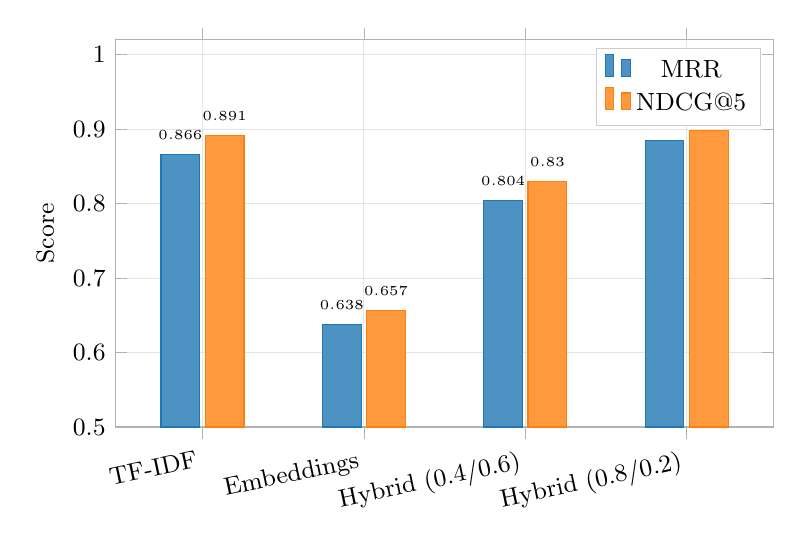
\begin{tikzpicture}
\begin{axis}[
  ybar,
  bar width         = 14pt,
  width             = 0.82\textwidth,
  height            = 6.5cm,
  enlarge x limits  = 0.18,
  ylabel            = {Score},
  ylabel style      = {font=\small},
  ymin=0.5, ymax=1.02,
  ytick             = {0.5,0.6,0.7,0.8,0.9,1.0},
  yticklabel style  = {font=\small},
  symbolic x coords = {TF-IDF, Embeddings, Hybrid (0.4/0.6), Hybrid (0.8/0.2)},
  xtick             = data,
  xticklabel style  = {font=\small, rotate=12, anchor=north east},
  legend style      = {at={(0.98,0.98)}, anchor=north east, font=\small,
                       draw=gray!40, fill=white},
  legend columns    = 1,
  nodes near coords,
  nodes near coords style = {font=\tiny, yshift=2pt},
  every node near coord/.append style={/pgf/number format/.cd, fixed, precision=3},
  grid              = major,
  grid style        = {draw=gray!20},
  axis line style   = {draw=gray!60},
  tick style        = {draw=gray!60},
]
\addplot[fill=tfidfblue!80, draw=tfidfblue]
  coordinates {
    (TF-IDF,0.8661)
    (Embeddings,0.6375)
    (Hybrid (0.4/0.6),0.8036)
    (Hybrid (0.8/0.2),0.8851)
  };
\addplot[fill=embedorange!80, draw=embedorange]
  coordinates {
    (TF-IDF,0.8911)
    (Embeddings,0.6565)
    (Hybrid (0.4/0.6),0.8297)
    (Hybrid (0.8/0.2),0.8982)
  };
\legend{MRR, NDCG@5}
\end{axis}
\end{tikzpicture}
\caption{MRR and NDCG@5 for each retrieval configuration. The optimal
         hybrid ($\alpha$=0.8, $\beta$=0.2) achieves the highest scores
         on both metrics.}
\label{fig:main_results}
\end{figure}

TF-IDF outperforms embeddings by a margin of 0.23 MRR points. The default
hybrid configuration — which weighted embeddings more heavily — actually
underperforms TF-IDF alone. This result was unexpected and motivated the
weight tuning experiment described in Section~\ref{sec:tuning}.

\subsection{Performance by Query Language}

Table~\ref{tab:bylang} and Figure~\ref{fig:lang_results} break MRR down
by query language pattern.

\begin{table}[H]
\centering
\caption{MRR by query language pattern.}
\label{tab:bylang}
\begin{tabular}{lccc}
\toprule
\textbf{Mode} & \textbf{Kinyarwanda} & \textbf{English} & \textbf{Mixed} \\
\midrule
TF-IDF     & 0.8094 & 0.8611 & 0.9278 \\
Embeddings & 0.4071 & 0.7939 & 0.7116 \\
Hybrid ($\alpha$=0.4, $\beta$=0.6) & 0.7419 & 0.8483 & 0.8206 \\
\bottomrule
\end{tabular}
\end{table}

% --- Figure: By-language grouped bar chart ---
\begin{figure}[H]
\centering
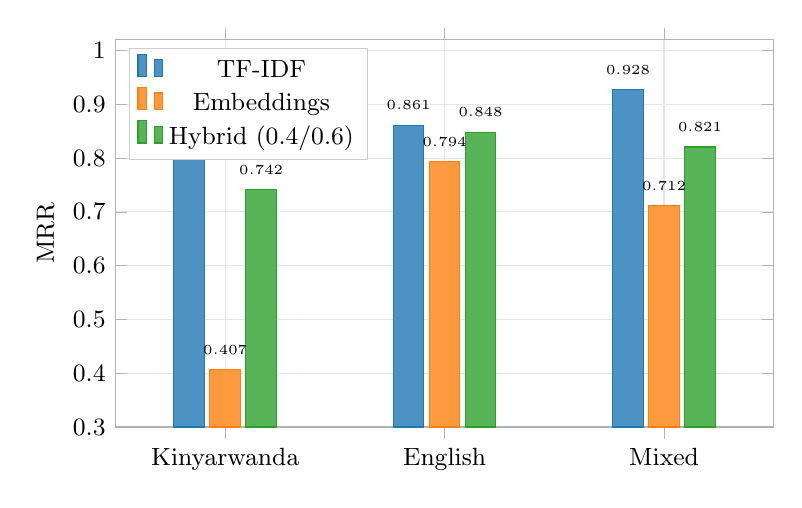
\begin{tikzpicture}
\begin{axis}[
  ybar,
  bar width         = 11pt,
  width             = 0.82\textwidth,
  height            = 6.5cm,
  enlarge x limits  = 0.25,
  ylabel            = {MRR},
  ylabel style      = {font=\small},
  ymin=0.3, ymax=1.02,
  ytick             = {0.3,0.4,0.5,0.6,0.7,0.8,0.9,1.0},
  yticklabel style  = {font=\small},
  symbolic x coords = {Kinyarwanda, English, Mixed},
  xtick             = data,
  xticklabel style  = {font=\small},
  legend style      = {at={(0.02,0.98)}, anchor=north west, font=\small,
                       draw=gray!40, fill=white},
  legend columns    = 1,
  nodes near coords,
  nodes near coords style = {font=\tiny, yshift=2pt},
  every node near coord/.append style={/pgf/number format/.cd, fixed, precision=3},
  grid              = major,
  grid style        = {draw=gray!20},
  axis line style   = {draw=gray!60},
  tick style        = {draw=gray!60},
]
\addplot[fill=tfidfblue!80, draw=tfidfblue]
  coordinates {(Kinyarwanda,0.8094)(English,0.8611)(Mixed,0.9278)};
\addplot[fill=embedorange!80, draw=embedorange]
  coordinates {(Kinyarwanda,0.4071)(English,0.7939)(Mixed,0.7116)};
\addplot[fill=hybridgreen!80, draw=hybridgreen]
  coordinates {(Kinyarwanda,0.7419)(English,0.8483)(Mixed,0.8206)};
\legend{TF-IDF, Embeddings, Hybrid (0.4/0.6)}
\end{axis}
\end{tikzpicture}
\caption{MRR broken down by query language pattern. The embedding
         retriever's sharp drop on Kinyarwanda queries (0.41) versus
         English queries (0.79) quantifies the cost of low-resource
         underrepresentation in multilingual pretraining.}
\label{fig:lang_results}
\end{figure}

The embedding retriever's collapse on Kinyarwanda queries — MRR of 0.41,
compared to 0.79 on English — is the most significant finding in this
work. The gap of 0.39 MRR points between languages, within the same
model, quantifies the cost of low-resource language underrepresentation
in multilingual pretraining corpora. Notably, TF-IDF achieves its highest
MRR on mixed queries (0.93), suggesting that English anchor words present
in code-switched queries provide strong lexical signals that benefit sparse
retrieval disproportionately.

\subsection{Weight Tuning}
\label{sec:tuning}

We evaluated nine hybrid configurations by varying $\alpha$ from 0.1 to
0.9 in increments of 0.1, with $\beta = 1 - \alpha$. Results are reported
in Table~\ref{tab:tuning} and Figure~\ref{fig:tuning}.

\begin{table}[H]
\centering
\caption{Hybrid weight tuning results. Bold denotes the optimal configuration.}
\label{tab:tuning}
\begin{tabular}{cccc}
\toprule
$\alpha$ (TF-IDF) & $\beta$ (Embedding) & \textbf{MRR} & \textbf{NDCG@5} \\
\midrule
0.1 & 0.9 & 0.6643 & 0.6790 \\
0.2 & 0.8 & 0.7186 & 0.7494 \\
0.3 & 0.7 & 0.7719 & 0.7923 \\
0.4 & 0.6 & 0.8036 & 0.8297 \\
0.5 & 0.5 & 0.8377 & 0.8554 \\
0.6 & 0.4 & 0.8650 & 0.8748 \\
0.7 & 0.3 & 0.8831 & 0.8907 \\
\textbf{0.8} & \textbf{0.2} & \textbf{0.8851} & \textbf{0.8982} \\
0.9 & 0.1 & 0.8724 & 0.8843 \\
\bottomrule
\end{tabular}
\end{table}

% --- Figure: Weight tuning line chart ---
\begin{figure}[H]
\centering
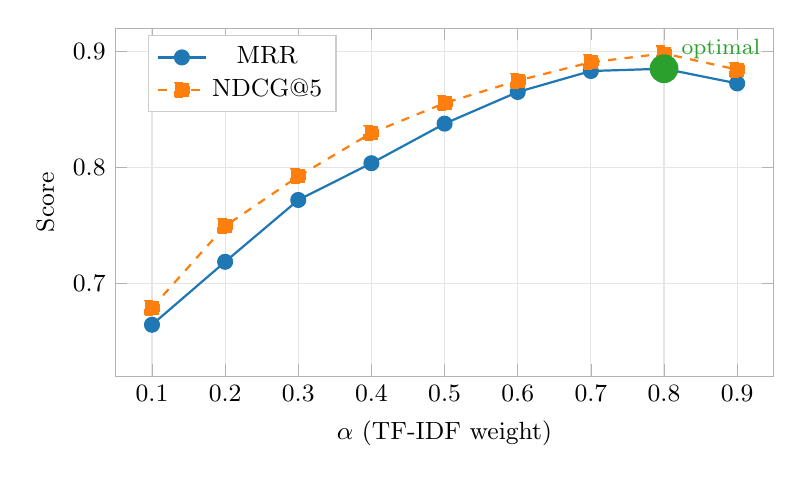
\begin{tikzpicture}
\begin{axis}[
  width             = 0.82\textwidth,
  height            = 6cm,
  xlabel            = {$\alpha$ (TF-IDF weight)},
  ylabel            = {Score},
  xlabel style      = {font=\small},
  ylabel style      = {font=\small},
  xmin=0.05, xmax=0.95,
  ymin=0.62, ymax=0.92,
  xtick             = {0.1,0.2,0.3,0.4,0.5,0.6,0.7,0.8,0.9},
  xticklabel style  = {font=\small},
  yticklabel style  = {font=\small},
  legend style      = {at={(0.05,0.98)}, anchor=north west,
                       font=\small, draw=gray!40, fill=white},
  legend columns    = 1,
  grid              = major,
  grid style        = {draw=gray!20},
  axis line style   = {draw=gray!60},
  tick style        = {draw=gray!60},
  mark size         = 2.5pt,
]
% MRR line
\addplot[
  color=tfidfblue, thick, mark=*, mark options={fill=tfidfblue}
] coordinates {
  (0.1,0.6643)(0.2,0.7186)(0.3,0.7719)(0.4,0.8036)
  (0.5,0.8377)(0.6,0.8650)(0.7,0.8831)(0.8,0.8851)(0.9,0.8724)
};
% NDCG@5 line
\addplot[
  color=embedorange, thick, mark=square*, mark options={fill=embedorange},
  dashed
] coordinates {
  (0.1,0.6790)(0.2,0.7494)(0.3,0.7923)(0.4,0.8297)
  (0.5,0.8554)(0.6,0.8748)(0.7,0.8907)(0.8,0.8982)(0.9,0.8843)
};
% Optimal marker
\addplot[
  color=hybridgreen, only marks, mark=*, mark size=5pt,
  mark options={fill=hybridgreen, draw=hybridgreen}
] coordinates {(0.8,0.8851)};
\node[font=\footnotesize, text=hybridgreen, anchor=south west]
  at (axis cs:0.8,0.8851) {~optimal};
\legend{MRR, NDCG@5}
\end{axis}
\end{tikzpicture}
\caption{MRR and NDCG@5 as a function of the TF-IDF weight $\alpha$.
         Both metrics rise monotonically until $\alpha$=0.8, then
         slightly decline — confirming a small but real contribution
         from the embedding component even at low weight.}
\label{fig:tuning}
\end{figure}

MRR increases monotonically as TF-IDF weight increases, peaking at
$\alpha=0.8$, $\beta=0.2$ with MRR=0.8851 and NDCG@5=0.8982. The slight
drop at $\alpha=0.9$ confirms a small but real contribution from semantic
embeddings even in this low-resource setting — the optimal hybrid
outperforms pure TF-IDF by 0.019 MRR points.

\subsection{Failure Analysis}
\label{sec:failure}

Four queries produced complete failures — the correct product did not
appear in the top 10 results under any configuration:

\begin{itemize}[leftmargin=1.5em, itemsep=2pt]
  \item \textit{``igiciro cya mudasobwa''} (price of a laptop) —
        \textit{igiciro} (price) does not appear in product descriptions,
        which characterize features rather than discuss pricing.
  \item \textit{``impuzu nziza za gabo''} (good clothes for men) —
        \textit{impuzu} (clothes) matches many fashion products equally,
        providing insufficient discriminative signal.
  \item \textit{``matelas nziza kuri igitanda''} (good mattress for a bed)
        — the mattress product name does not contain \textit{igitanda}
        (bed), breaking the lexical link.
  \item \textit{``ndashaka wardrobe nini y'icyumba''} (I want a big
        wardrobe for the room) — modifier noise from \textit{nini}
        (big) and \textit{y'icyumba} (of the room) suppressed the
        correct product's score below retrieval threshold.
\end{itemize}

An additional ten queries returned the correct product outside rank 1.
The most common pattern was high-frequency Kinyarwanda terms
(\textit{nziza, ndashaka}) inflating similarity scores for semantically
unrelated products that happen to share common vocabulary — a
Kinyarwanda-specific variant of the IDF failure mode.

% ============================================================
% SECTION 6 — CONCLUSION
% ============================================================
\section{Conclusion}
\label{sec:conclusion}

This paper set out to answer a question that most multilingual NLP
research has not bothered to ask: what happens when you build a search
engine for a population that actually code-switches, using a language
that pretraining corpora have largely ignored?

KinyaSearch demonstrates that hybrid retrieval — combining sparse lexical
matching with dense semantic embeddings — is an effective architecture for
Kinyarwanda-English e-commerce search, achieving MRR=0.89 and NDCG@5=0.90
at optimal configuration. This represents a meaningful baseline for a
problem that had no prior benchmark.

But the more interesting result is the one that complicates the prevailing
narrative. Multilingual sentence embeddings, widely assumed to generalize
across languages, achieve an MRR of 0.41 on pure Kinyarwanda queries — a
number that should give pause to anyone deploying off-the-shelf
multilingual models in low-resource African language settings without
empirical validation. TF-IDF, a method decades older, outperforms it
substantially. The optimal hybrid weights this classical method at 80\%.

Several directions remain open. Fine-tuning the embedding model on
Kinyarwanda product descriptions — even a small in-domain corpus — would
likely close much of the performance gap. Expanding the dataset to
thousands of real product listings scraped from live Rwandan platforms
would produce a more ecologically valid benchmark. Incorporating user
interaction data — click-through rates, session logs — would allow
learning-to-rank approaches that go beyond the unsupervised methods used
here. And extending the system to handle voice queries, increasingly
common on low-bandwidth mobile connections, would address a real deployment
constraint in the Rwandan market.

The dataset, code, and evaluation scripts are fully open. We hope this
work provides a foundation — however modest — for the researchers who
come next.

% ============================================================
% REFERENCES
% ============================================================
\bibliographystyle{plainnat}
\begin{thebibliography}{99}

\bibitem[Alabi et al.(2022)]{alabi2022}
Alabi, J.~O., Adelani, D.~I., Mesham, M., \& Bassett, B.~A. (2022).
Adapting pretrained language models to African languages via multilingual
adaptive fine-tuning.
\textit{Proceedings of COLING 2022}.

\bibitem[Asai et al.(2021)]{asai2021}
Asai, A., Kasai, J., Clark, J., \& Hajishirzi, H. (2021).
XOR QA: Cross-lingual open-retrieval question answering.
\textit{Proceedings of NAACL 2021}.

\bibitem[Feng et al.(2022)]{feng2022}
Feng, F., Yang, Y., Cer, D., Arivazhagan, N., \& Wang, W. (2022).
Language-agnostic BERT sentence embedding.
\textit{Proceedings of ACL 2022}.

\bibitem[Formal et al.(2021)]{formal2021}
Formal, T., Piwowarski, B., \& Clinchant, S. (2021).
SPLADE: Sparse lexical and expansion model for first stage ranking.
\textit{Proceedings of SIGIR 2021}.

\bibitem[Gupta et al.(2021)]{gupta2021}
Gupta, S., Chatterjee, A., \& Pal, U. (2021).
Code-mixed information retrieval for Hindi-English queries.
\textit{Proceedings of FIRE 2021}.

\bibitem[Jose et al.(2020)]{jose2020}
Jose, N., Ravishankar, V., \& Haffari, G. (2020).
Cross-lingual transfer learning for Tamil-English code-switched search.
\textit{Findings of EMNLP 2020}.

\bibitem[Longpre et al.(2023)]{longpre2023}
Longpre, S., Yauney, G., Reif, E., et al. (2023).
A pretrainer's guide to training data: Measuring the effects of data age,
domain coverage, quality, and toxicity.
\textit{arXiv:2305.13169}.

\bibitem[Nekoto et al.(2020)]{nekoto2020}
Nekoto, W., Marivate, V., Matsila, T., et al. (2020).
Participatory research for low-resourced machine translation: A case study
in African languages.
\textit{Findings of EMNLP 2020}.

\bibitem[Nie et al.(1999)]{nie1999}
Nie, J.~Y., Simard, M., Isabelle, P., \& Durand, R. (1999).
Cross-language information retrieval based on parallel texts and automatic
mining of parallel texts from the web.
\textit{Proceedings of SIGIR 1999}.

\bibitem[Reimers \& Gurevych(2019)]{reimers2019}
Reimers, N., \& Gurevych, I. (2019).
Sentence-BERT: Sentence embeddings using Siamese BERT-networks.
\textit{Proceedings of EMNLP 2019}.

\bibitem[Zhang et al.(2021)]{zhang2021}
Zhang, X., Oguz, B., Karpukhin, V., et al. (2021).
Multilingual open-domain question answering with unified dense retrieval.
\textit{arXiv:2107.11976}.

\end{thebibliography}

\end{document}